\documentclass[twocolumn]{article}

\def\topfraction{.85}
\def\dbltopfraction{.85}
\def\textfraction{.12}

\usepackage{natbib}
\usepackage{amsmath}
\usepackage[utf8]{inputenc}
\usepackage{graphicx}
\usepackage{url}
% \usepackage{subequations}

\def\npup{\ensuremath{U}}
\def\nmaj{\ensuremath{M}}
\def\nprof{\ensuremath{S}}
\def\ngrad{\ensuremath{P}}
\def\ngrant{\ensuremath{G}}
\def\nisi{\ensuremath{P^\text{I}}}
\def\nscielo{\ensuremath{P^\text{S}}}

\def\der#1#2{\frac{\mathrm{d}\,{#1}}{\mathrm{d}#2}}
\def\pder#1#2{\frac{\partial\,{#1}}{\partial#2}}

\def\nal{\ensuremath{N_\text{pub}}}
\def\nal{\ensuremath{N_\text{alumnos}}}
\def\nal{\ensuremath{N_\text{alumnos}}}
\def\eqref#1{Eq.~(\ref{eq:#1})}
\makeatletter
\def\eqsref#1#2{Eqs.~(\ref{eq:#1}--\ref{eq:#2})}
\makeatother

\usepackage{geometry}
\geometry{left=16mm,top=16mm,right=20mm,bottom=20mm}

\title{Direct State funding of Chilean universities}
\author{Régis Lachaume}

\begin{document}

\maketitle

\section{Calculation}
\subsection{Yearly evaluation}
\subsubsection{Determination}
\label{sec:metrics}

Art. 2 of Decree with Force of Law 4 of 1980, with modifications from Art. 1 of Ministry of Education Decree 116 of 2002, indicates that 5\% part of the total funding of year $n + 1$ is distributed to University $i$ according to its metrics measured in year $n$. They involve 
\begin{itemize}
\item $\npup_{i,n}$, the number of undergraduate students (``estudiantes de pregrado'');
\item $\nmaj_{i,n}$, the number of majors (``carreras'');
\item $\nprof_{i,n}$, the number of equivalent full-time scholars (``académicos''), i.e. professors and researchers;
\item $\ngrad_{i,n}$, the number of equivalent full-time scholars with a post-graduate title such as master or a PhD; 
\item $\ngrant_{i,n}$, the number of research grants (``proyectos'');
\item $\nisi_{i,n}$, the number of Web of Science publications (WoS)\footnote{At the time of the Decree 116 it was known as ISI}; 
\item and $\nscielo_{i,n}$, the number of non-WoS publications indexed by the Scientific Electronic Library Online (Scielo) Chile. 
\end{itemize}

The metrics, defined in the aformentioned decrees, are ratios meant to measure an output v. staff efficiency\footnote{While the number of publications is defined by the number of WoS plublications plus one third of Scielo one by Ministry of Education Decree 116 of 2002, the Ministry has consistently used factor 0.33 instead of 1/3 for the calculation.}
\begin{subequations}
\begin{align}
    x_{i,n,1} &= \npup_{i,n} / \nmaj_{i,n},  \label{eq:x1}                          \\
    x_{i,n,2} &= \npup_{i,n} / \nprof_{i,n},                           \\ 
    x_{i,n,3} &= \ngrad_{i,n} / \nprof_{i,n},                          \\
    x_{i,n,4} &= \ngrant_{i,n} / \nprof_{i,n},                         \\
    x_{i,n,5} &= (\nisi_{i,n} + \frac{33}{100} \nscielo_{i,n}) / \nprof_{i,n}
\end{align}
\end{subequations}

According to Art. 3 of Ministry of Education Decree 128 of 1991,  the
evaluation formula renormalises the aforemention ratios in this
way\footnote{Although not specified by the decree, the Ministry has
consistently used the population variance, not the sample variance, for the calculation.}:
\begin{subequations}
\begin{align}
    \mu_{n,k}    &= \frac1N\sum_j x_{j,n,k}\qquad\text{(mean)} \label{eq:mu}\\
    \sigma_{n,k} &= \sqrt{\frac 1N \Big(\sum_j x_{j,n,k}^2\Big) - N\mu_{n,k}^2}\qquad\text{(std. dev.)} \label{eq:sigma}\\
    \xi_{i,n,k}  &= \frac{x_{i,n,k} - \mu_{n,k} }{\sigma_{n,k}} 
\qquad\text{(reduced coeff.)} \label{eq:xi}\\
    y_{i,n,k}    &= \exp \left[ -\frac 75 + \frac{\xi_{i,n,k}}4  \right]^3 \label{eq:transform}
\end{align}
\end{subequations}
where $N$ is the total number of universities.
The transform in \eqref{xi} ensures that Universities are compared by how much they deviate from the mean. The exponential in \eqref{transform} is supposed to simulate a biological growth. Figure~\ref{fig:transform} displays the exponential nature of the rating.

\begin{table}[t]
\centering
\caption{Coefficients used for university evaluation since 1998.}
\label{tab:coeff}
\begin{tabular}{lll}
\hline\hline
      & ratio                   & value\\
\hline
$c_1$ & students-to-majors      & 0.01\\
$c_2$ & students-to-staff       & 0.14\\
$c_3$ & postgrad staff-to-staff & 0.24\\
$c_4$ & grants-to-staff         & 0.25\\
$c_5$ & papers-to-staff         & 0.35\\
\hline
\end{tabular}
\end{table}


Art. 2 of Decree with Force of Law 4 of 1980 indicates that 5\% of the funding
is indexed on a weighted average of the metrics $y_{i,n,k}$ (k in $1\cdots5$)
(see Sect.~\ref{sec:metrics}). The weights $c_k$ may vary from year to year,
but have been constant since 1998 (see Table~\ref{tab:coeff}).  University $i$
is thus assigned a score
\begin{subequations}
\begin{align}
    y_{i,n}    &= \sum_k c_k y_{i,n,k}. \label{eq:y}\\
\intertext{and, using the total score}
    y_{n}      &= \sum_i y_{i,n},\\
\intertext{a funding share}
    f_{i,n}    &= \frac{y_{i,n}}{y_{n}} \label{eq:f}
\end{align}
\end{subequations}


\begin{figure}[t]
\centering
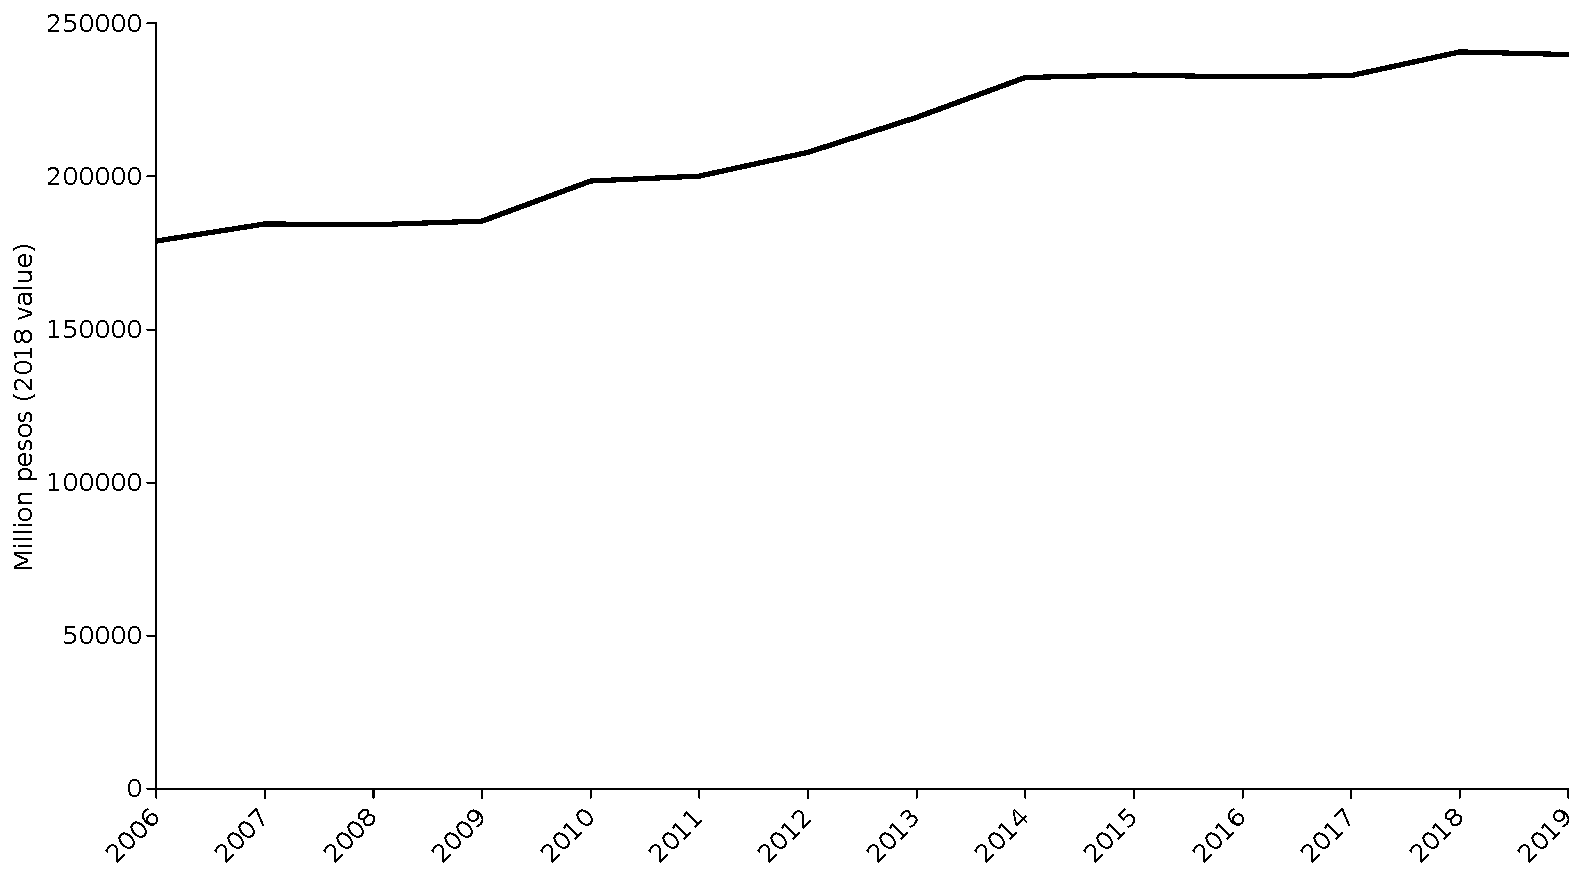
\includegraphics[width=\linewidth]{pdf/total-afd-timeseries.pdf}
\caption{Evolution of total direct State funding to Chilean Universities, in 2018
pesos (inflation-corrected).}
\label{fig:total-afd}
\end{figure}


\subsubsection{Marginal earnings}
\label{sec:marginal} 

In this section, we focus on a yearly snapshot and drop the $n$ index in the formulae.  We examine the case where university $i$ decides to increase one of its ratios number $k$ by a small number of standard deviations $\Delta\xi_{i,k}$, so that the ratio $x_{i,k}$ improves by $\Delta x_{i,k} = \sigma_k\Delta\xi_{i,k}$.

For any university $j$, the new value of the score $y_{j,k}$ is usually modified because the mean and standard deviation are changed via $x_{i,k}$.  The difference $\Delta y_{j,k}$ is given by differentiating \eqref{transform}, and in turn \eqsref{mu}{xi} on which it depends.
The calculation, detailed in  in Appendix~\ref{sec:calculus}, yields
\begin{equation}
    \frac{\Delta y_{j,k}}{y_{j,k}} = 
        \frac34 \left(\frac{\xi_{j,k}}4 -  \frac75\right)^2 
        \left(
            \delta_{ij} 
          - \frac 1N - \frac{\xi_{i,k}\xi_{j,k}}{N}
        \right)
        \Delta \xi_{i,k},
        \label{eq:modif}
\end{equation}
where $\delta_{ij} = 1$ if universities $i$ and $j$ are the same and zero otherwise.

The meaning of \eqref{modif} is the following:
\begin{enumerate}
    \item \emph{$(\xi_{j,k}/4 - 7/5)^2$ factor}:  The relative improvement depends on the relative standing of the University in the ranking.  A university lagging behind by 2 standards deviations gets a relative improvement 4,5 times higher than a university standing out by 2 standard deviations.
    \item \emph{$\delta_{ij}$ term:} University $i$ generally benefits from an increase of its own ratio $\Delta x_{i,k}$: the $\delta_{ij}$ (= 1 for $i = j$) term in the equation is the only one that is not in $1/N$. However, if $|\xi_{i,k}| > \sqrt{N - 1} \approx 5$ standard deviations, University could lose from improving.  Nevertheless, the data of the Ministery from 2006 to 2018 can be used to show that the highest deviation any of the ratio has ever reached is 3.7.
    \item University $j$ may benefit from, or be harmed by, the improvement of University $i$.  There are two effects at play.  
    \begin{enumerate}
    \item \emph{$1/N$ term}: The increase of the mean, would on its own hurt all other universities as their position relative to the mean $\xi_{j,k}$ would drop (see the $1/N$ term in the equation).  
    \item \emph{$\xi_{i,j}\xi_{j,k}/N$ term}: However, the modification of the standard deviation works both ways. Intuitively, if a university with a high $\xi_{i,k} > 0$ ($x_{i,k} > \mu_k$) improves, it will increase the standard deviation, so that all universities deviate less from the mean: other universities with $\xi_{j,k} > 0$ will lose some of their good standing and lower tier ones with $\xi_{j,k} < 0$ will decrease their lag . Conversely, on can see that the improvement of a University with a lower rank $\xi_{j,k} < 0$, by decreasing the standard deviation of the sample when it goes closer to the mean, will help those with good standing to stand out more and harm other lower tier ones. 
\end{enumerate}
    For both effects combined, University $j$ benefits if $\xi_{i,k}\xi_{j,k} < -1$ and is harmed otherwise. 
\end{enumerate}

To determine the additional funding fraction $\Delta f_j$, we propagate 
\eqref{modif} into \eqsref{y}{f}:
\begin{equation}
    \frac{\Delta f_j}{f_j} = c_k \left[
                     \left(1 - \frac{y_{j}}y\right)\frac{\Delta y_{j,k}}{y_{j}}
                    - \sum_{l \ne j} \frac{y_l}y \frac{\Delta y_{l,k}}{y_l}
                 \right].
\end{equation}
The first term in the square brackets has the same sign as $\Delta y_{j,k}$ because, by definition, $y_j < y$.  In most cases, the second term is smaller than the first one because the $\Delta y_{l,k}$ partially cancel out (some positives and some negatives) and $y_l < y$. It means that the funding received by a university that has an improved rating normally receives additional funding.  It is possible, though, that a university with a very small $\Delta y_{j,k}$ (e.g. $\xi_{j,k} < -2$) will be harmed by increasing its score, because the other, larger, $\Delta y_{l,k}$ coould lead to a second term larger than the first term under these circumstances.  In years 2006--2019 it has ocurred once, very marginally, in 2015, for Universidad de Talca.  It would have received 1,000 CLP less had it substituted four regular professors with ones owning a postgraduate degree (improvement of $y_{\text{U. Talca}, 2015, 3}$).  It happened on that year that Universidad de Talca had the highest negative standard deviation observed for any metrics in the period 2006--2019 ($\xi \approx -2.8$). 

\subsection{Time evolution}
\paragraph{Total funding}
The total funding in year $n$, that we note $F_{n}$, is a slowly increasing series (see Fig.~\ref{fig:total-afd}). In half of the years it approximately follows the consumer price index, but it has received a modest boost in other years.  The average inflation-corrected increase has been $2.3$\% per year in period 2006--2019. This increases matches the increase in undergraduate students ($+2.2\%$ in 2006--2018), real wages ($+2\%$?), and GDP per capita ($+2.xx$\%?). Increase in standard of living and student population are long-term trends that I would expect to hold for at least the next decade, so we can safely assume that University funding by the State will still follow this trend.

For predictions, beyond 2019, I will therefore assume that
\begin{equation}
    F_{n+1} = F_n (1 + q) \label{eq:F}
\end{equation}
where $q = 2$\%.

\paragraph{University funding}
Let $F_{i,n}$ be the funding received by university $i$ at year $n$. Art. 2 of
Decree with Force of Law 4 of 1980 indicates that 5\% of the funding is indexed
on metrics $y_{i,n,k}$ and 95\% of the funding is related to the previous year's
share of the total funding.  So,

\begin{align}
    F_{i,n+1} &= \left( \frac{19}{20} \frac{F_{i,n}}{F_{n}} 
                      + \frac 1{20} \frac{y_{i,n}}{\sum_j y_{j,n}} 
                \right) F_{n+1}.
        \label{eq:afd}
\end{align}


\subsection{Checks}
\begin{figure}
\centering
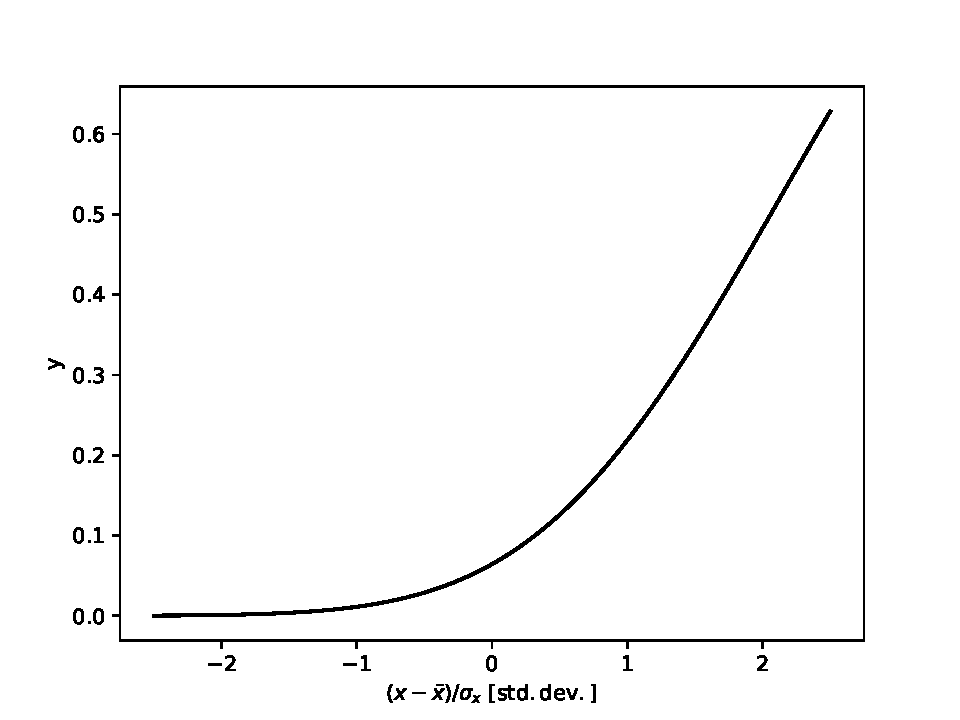
\includegraphics[width=.85\linewidth]{pdf/transform.pdf}
\caption{Transformation of the metric $x_{i,n,k}$ into $y_{i,n,k}$, before a weighted sum 
$\sum_k c_{i,n,k} y_{i,n,k}$ is performed to determine the rating of university $i$ in year $n$.}
\label{fig:transform}
\end{figure}

\paragraph{Yearly evaluation} I have checked the calculations of the 5\% using open data from the Eduction Ministry for
years 2006 to 2018. For each year since 2011 and 2007--2009, the percentages I
derived (see Table~\ref{tab:calcdetail} for 2018) match within numerical
rounding errors (8 digits) with those of the Ministry. The subsidies I predict
for each university differ by at most CLP 1,000 (USD 1.50) with the
official ones due to rounding errors, as the accounting unit used in the
official documents is 1,000 Chilean pesos. In 2010, the Ministry used the 2009
calculation with 2008 metrics, instead of 2009 ones, leading to large differences if the 2009 metrics given in the Ministry's spreadsheet is used.  Difference are zero within rounding errors using 2008 data instead. In 2006, there is an unexplained 0.01\% discrepancy between my determination and the Ministry's.  The official file from the ministry with added columns showing my calculations are available from github project \url{https://github.com/loqueelvientoajuarez/afd}.\footnote{The original ministry file can
be obtained from \url{http://dfi.mineduc.cl/usuarios/MECESUP/File/2018/instrumentos/AFD/AFD_2006_al_2018_MontosVariables5xc(1).xlsx} and my calculations from \url{https://github.com/loqueelvientoajuarez/afd/blob/master/src/tabla-afd.xlsx}}. 
The detail of calculations for year 2018 is given in Appendix.~\ref{sec:2018}.
For that year, my calculations match exactly the Ministery's to the peso.

\paragraph{Time-evolution} I have checked the recurrence formula \eqref{afd} using the total amount given for each year $F_n$.  The 95\% funding is well predicted from year to year, except again for 2010, where I had to substitude 2008 funding percentages to the expected 2009 ones. Because of rounding errors cumulating from year to year, the amounts I predict for 2018 differ by up to 7,000 pesos (approx USD 10) with those of the Ministry.

\paragraph{Marginal earnings}  Marginal earnings have been determined by two methods.  The first one, using differential calculus in Sect.~\ref{sec:marginal}, and the second one, by doing the full calculation with \eqref{afd} using the new values of the coefficients.  We have checked that both method agree within a few significant digits as long as the variations remain small.

\section{Value of an additional paper, project, or staff}
\begin{table*}[t]
\centering
\caption{Additional earnings in 2019 Chilean pesos for thes marginal improvement of 2018 metrics: an additional one-year contract of a postgraduate professor, an additional one-year research grant, and an additional Web of Science publication.  2019 funding is accurate to 1,000 pesos. The total funding assumed that the State funding increases 2\% a year real terms.  A research grant typically lasts 3 years and will carry the same level of funding for each year it is active.  An additional tenure-track/tenured professor will bring as much funding as the years they stay hired.}
\label{tab:sciencecost}
\begin{tabular}{l rr rr rr}
\hline\hline
universidad                    & \multicolumn{2}{c}{postgraduate staff} & \multicolumn{2}{c}{research grant} & \multicolumn{2}{c}{WoS publication} \\
                               & 2019        & all years     & 2019        & all years     & 2019        & all years     \\
                               & [CLP]       & [CLP]         & [CLP]       & [CLP]         & [CLP]       & [CLP]         \\
\hline
U. de Chile                    &     303\,000 &     9\,774\,194 &     952\,000 &    30\,709\,677 &     517\,000 &    16\,677\,419 \\
P. U. Católica de Chile        &     330\,000 &    10\,645\,161 &     981\,000 &    31\,645\,161 &     531\,000 &    17\,129\,032 \\
U. de Concepción               &   1\,098\,000 &    35\,419\,355 &   1\,104\,000 &    35\,612\,903 &     640\,000 &    20\,645\,161 \\
U. Católica de Valparaíso      &   2\,902\,000 &    93\,612\,903 &   3\,229\,000 &   104\,161\,290 &   1\,753\,000 &    56\,548\,387 \\
U. Téc. Federico Sta.Maria     &     505\,000 &    16\,290\,323 &   2\,397\,000 &    77\,322\,581 &   1\,378\,000 &    44\,451\,613 \\
U. de Santiago                 &     316\,000 &    10\,193\,548 &     960\,000 &    30\,967\,742 &     418\,000 &    13\,483\,871 \\
U. Austral                     &   1\,128\,000 &    36\,387\,097 &   1\,286\,000 &    41\,483\,871 &     798\,000 &    25\,741\,935 \\
U. Católica del Norte          &     302\,000 &     9\,741\,935 &     818\,000 &    26\,387\,097 &     964\,000 &    31\,096\,774 \\
U. de Valparaíso               &     657\,000 &    21\,193\,548 &   1\,014\,000 &    32\,709\,677 &     357\,000 &    11\,516\,129 \\
U. de Antofagasta              &   1\,285\,000 &    41\,451\,613 &     916\,000 &    29\,548\,387 &   1\,102\,000 &    35\,548\,387 \\
U. de la Serena                &     227\,000 &     7\,322\,581 &   1\,008\,000 &    32\,516\,129 &   1\,376\,000 &    44\,387\,097 \\
U. de Bio Bio                  &   4\,045\,000 &   130\,483\,871 &   1\,108\,000 &    35\,741\,935 &     669\,000 &    21\,580\,645 \\
U. de la Frontera              &   2\,378\,000 &    76\,709\,677 &   4\,705\,000 &   151\,774\,194 &   2\,781\,000 &    89\,709\,677 \\
U. de Magallanes               &   2\,847\,000 &    91\,838\,710 &   3\,108\,000 &   100\,258\,065 &   3\,023\,000 &    97\,516\,129 \\
U. de Talca                    &   3\,828\,000 &   123\,483\,871 &   3\,177\,000 &   102\,483\,871 &   1\,054\,000 &    34\,000\,000 \\
U. de Atacama                  &      20\,000 &       645\,161 &     323\,000 &    10\,419\,355 &     384\,000 &    12\,387\,097 \\
U. de Tarapacá                 &   5\,596\,000 &   180\,516\,129 &   1\,485\,000 &    47\,903\,226 &   2\,178\,000 &    70\,258\,065 \\
U. Arturo Prat                 &     137\,000 &     4\,419\,355 &     439\,000 &    14\,161\,290 &      97\,000 &     3\,129\,032 \\
U. Metropolitana               &   1\,960\,000 &    63\,225\,806 &     272\,000 &     8\,774\,194 &      89\,000 &     2\,870\,968 \\
U. de Playa Ancha              &   3\,762\,000 &   121\,354\,839 &   1\,180\,000 &    38\,064\,516 &     209\,000 &     6\,741\,935 \\
U. Tecnológica Metropolitana   &     451\,000 &    14\,548\,387 &     519\,000 &    16\,741\,935 &     250\,000 &     8\,064\,516 \\
U. de Los Lagos                &     886\,000 &    28\,580\,645 &     723\,000 &    23\,322\,581 &     227\,000 &     7\,322\,581 \\
U. Católica de Maule           &   1\,918\,000 &    61\,870\,968 &     544\,000 &    17\,548\,387 &     343\,000 &    11\,064\,516 \\
U. Católica de Temuco          &   1\,583\,000 &    51\,064\,516 &     574\,000 &    18\,516\,129 &     192\,000 &     6\,193\,548 \\
U. C.de la Sant.Concepción     &     712\,000 &    22\,967\,742 &     571\,000 &    18\,419\,355 &     325\,000 &    10\,483\,871 \\
U. de O'Higgins                &  22\,842\,000 &   736\,838\,710 &  12\,518\,000 &   403\,806\,452 &   8\,501\,000 &   274\,225\,806 \\
U. de Aysén                    &  81\,972\,000 & 2\,644\,258\,065 &  64\,904\,000 & 2\,093\,677\,419 &   9\,284\,000 &   299\,483\,871 \\
\hline
\end{tabular}
\end{table*}



If an additional paper is published by a researcher of University $i$ in year $n$, it will reflect in 
the 5\% funding of year $n + 1$. Let us call $\Delta F_{i,n+1}$ the additional earnings 
of the university in that year.  In the subsequent years, it will reflect via the 95\% 
(first term of the right handside of \eqref{afd}) in this way:
\begin{align}
   \Delta F_{i,n+k} &=  \frac{19}{20} \Delta F_{n+k-1} F_{n+k}  / F_{n+k-1}, \notag\\
\intertext{so, using \eqref{F},}
   \Delta F_{i,n+k} &= \Delta F_{n+k-1}  \frac{ 19 (1 + q)} { 20}
\end{align}

The additional funding obtained by the university in all years is therefore
\begin{align}
    \Delta F_{i} &= \sum_{k=1}^{+\infty} \Delta F_{i,n+k} \notag \\
                 &= \sum_{k=1}^{+\infty} \frac{19(1 + q)}{20} \,\Delta F_{i,n+1} \notag \\
                 &= \frac{20} { 1 - 19q } \Delta F_{i,n+1}\\
                 &\approx 32 \Delta F_{i,n+1}. \notag
\end{align}

The determination of $\Delta F_{i,n+1}$ is straightforward.  The calculations
in \eqsref{x1}{afd}) are done with the metrics provided by the Ministry (see Sect.~\ref{sec:metrics}) and for the same ones with an additional publication.  The difference in funding is $\Delta F_{i,n+1}$. 

Table~\ref{tab:sciencecost} gives the 2019 funding a University would have received, had an additional 2019 paper been published, an additional one-year science staff (professor) been contracted, or an additional grant been obtained (postdoct staff or other project).  I have made the hypothesis, that no other Traditional University has co-authored the paper, in which case the amount may vary. 

My figures are much larger than those derived by \citet{RAM12}.  The reasons are that they
\begin{enumerate}
\item only consider the first five years after the paper is published while the half-life of the 95\% dampening is 14 years, meaning that they underestimate the total revenue obtained with a paper by a factor of $\approx 4$
\item include an additional dampening of 8\% per year that they do not justify and is not based on any kind of calculation by the Ministry, meaning that they underestimate the additional funding by a factor of $\approx 2.5$ to 4;\footnote{Quite the contrary, the constant increase of the total funding (consumer price index +2\%) calls for an amplification of 2\%}
\item use 2010 data, meaning that the monetary incentive is larger than the 2018 one by a factor of $\approx 2$; and
\item seem to use different values for the coefficients than those retroactively published in 2012. Their Fig.~4 doesn't match the corrected coefficients we derive for 2009, 2010, or 2011. Actually, both our data and Ministry's figures for years 2006 to 2017 show a systematic discrepancy between U. de Chile and P. U. Católica de Chile of the order of 25-35\%  in weighted sum of corrected coefficients and share of the 5\%, while their Figure gives about 10\%.
\end{enumerate}

\appendix
\section{Derivation of equation}
\label{sec:calculus}
The variation in $\Delta y_{j,k}$ is linked to $\Delta \xi_{i,k}$ via the
derivative:
\begin{align}
    \Delta y_{j,k} 
        &\approx \pder{y_{j,k}}{x_{i,k}}
                 \, \Delta x_{i,k},\\
        &\approx \der{y_{j,k}}{\xi_{i,k}}
                 \, \pder{\xi_{i,k}}{x_{i,k}}
                 \, \sigma_k \Delta \xi_{i,k},\\
\intertext{so, substituting \eqref{xi}, for the second factor}
        &\approx \der{y_{j,k}}{\xi_{i,k}}
                 \left[
                    \pder{x_{j,k}}{x_{i,k}}
                  - \pder{\mu_k}{x_{i,k}} 
                  - \frac{x_{j,k}-\mu_k}{\sigma_k}\pder{\sigma_k}{x_{i,k}} 
                 \right] 
                 \, \Delta \xi_{i,k}\\
\intertext{and, backsubstituting \eqref{xi},}
        &\approx \der{y_{j,k}}{\xi_{i,k}}
                 \left[
                    \pder{x_{j,k}}{x_{i,k}}
                  - \pder{\mu_k}{x_{i,k}}
                  - \xi_{j,k} \pder{\sigma_k}{x_{i,k}}
                 \right]
                 \, \Delta \xi_{i,k}.
\end{align}

The first factor is the derivative of the function in the right handside of Eq.~(\ref{eq:transform}). It is:
\begin{equation}
    \der{y_{i,k}}{\xi_{i,k}} = \frac34 \left[ -\frac75 + \frac{\xi_{i,k}}4 \right] y_{i,k}.
\end{equation}

In the second factor, the first term is one if $i = j$, $x_{j,k}$ and $x_{i,k}$ being then the same variable, and zero otherwise.  The second term is the variation of the mean when one of the term varies, it is therefore $1/N$ the variation of the individual term. So,
\begin{align}
    \pder{x_{j,k}}{x_{i,k}} &= \delta_{ij}, \label{eq:derx}\\
    \pder{\mu_k}{x_{i,k}}   &= \frac 1N \sum_j \pder{x_{j,k}}{x_{i,k}}
                             = \frac 1N \sum_j \delta_{ij}
                             = \frac 1N. \label{eq:dermu}
\end{align}

The last term requires some more calculation. We use \eqref{sigma}:
\begin{align}
    \pder{\sigma_k}{x_{i,k}}
        &= \pder{}{x_{i,k}} \sqrt{\frac 1N \Big(\sum_j x_{j,n,k}^2\Big) - \mu_{n,k}^2},\\
        &= \frac 1{2\sigma_k} \pder{}{x_{i,k}} 
            \left[ 
                \frac 1N \Big(\sum_j x_{j,k}^2\Big) - \mu_k^2
            \right],\\
        &= \frac 1{2\sigma_k} 
            \left[
                \frac 2N \sum_k x_{j,k} \pder{x_{j,k}}{x_{i,k}} 
                - 2 \mu_k \pder{\mu_k}{x_{i,k}}
            \right],\\
\intertext{so, using \eqref{derx} and \eqref{dermu},}
        &= \frac 1{2\sigma_k}
            \left[
                \frac {2\xi_{i,k}}{N} - \frac{2\mu_k}{N}
            \right]
\intertext{and, finally, with \eqref{xi},}
        &= \frac{\xi_{i,k}}N.
\end{align}

\section{Direct state funding in 2018}
\label{sec:2018}

Table~\ref{tab:metrics} and \ref{tab:calcdetail} show the metrics used by the
Ministry in 2018 and the calculation details for $x_k$ and $y_k$. 

\begin{table*}[t]
\caption{Metrics used for the Direct State funding (aporte fiscal directo) of
main Chilean Universities in 2018. \npup{}, the number of
undergrad students; \nmaj{}, the number of majors; \nprof{}, the number of
(equivalent) full-time professors and researchers (``académico''); \ngrad{},
the number of (equivalent) full-time staff with post-graduate title; \ngrant{},
the number of research grants; $\nisi$, the number of ISI publications; and
$\nscielo$, the number of non-ISI publications indexed by the Scientif
Electronic Library Online Chile.}
\label{tab:metrics}
\centering\footnotesize
\begin{tabular}{l rrrrrrr}
\hline
University                 & \npup  & \nmaj &\nprof  &\ngrad &\ngrant& \nisi&\nscielo\\
\hline\hline
U. de Chile               & 30480 	& 77 &   2236.64&1499.84&855.5  &  2305&	279  \\
P. U. Católica de Chile    & 26767 	& 76 &   2232.60&1508.94&763.0  &  2171&	237  \\
U. de Concepción           & 24666 	& 90 &   1432.16&1129.67&388.0  &  1050&	121  \\
U. Católica de Valparaíso  & 14121 	& 52 &    633.04& 518.95&209.0  &   545&	 69  \\
U. Téc. Fedérico Sta. María& 15105 	& 77 &    677.03& 405.92&169.0  &   522&	  6  \\
U. de Santiago             & 18645 	& 68 &   1122.57& 695.14&210.0  &   565&	 58  \\
U. Austral                 & 13218 	& 60 &    911.62& 628.02&184.0  &   534&	 66  \\
U. Católica del Norte      & 10407 	& 52 &    590.90& 362.66& 63.0  &   328&	 34  \\
U. de Valparaíso           & 14737 	& 60 &    873.13& 557.72&120.0  &   409&	 42  \\
U. de Antofagasta          &  6369 	& 56 &    399.75& 256.79& 39.0  &   207&	 11  \\
U. de la Serena            &  7084 	& 41 &    370.42& 209.56& 28.0  &   165&	 14  \\
U. de Bio Bio              & 11028 	& 62 &    498.67& 426.73& 66.0  &   198&	 26  \\
U. de la Frontera          &  9346 	& 48 &    423.96& 300.01&160.0  &   450&	 40  \\
U. de Magallanes           &  2962 	& 27 &    268.08& 129.13& 27.0  &   106&	 15  \\
U. de Talca	               &  9342 	& 41 &    465.00& 427.80&124.0  &   312&	 43  \\
U. de Atacama              &  6359 	& 71 &    317.73& 138.05&  5.0  &    78&	  3  \\
U. de Tarapacá             &  8525 	& 63 &    358.23& 305.34& 36.0  &   248&	 32  \\
U. Arturo Prat             &  4326 	& 39 &    441.08& 227.30& 16.0  &    52&	 18  \\
U. Metropolitana           &  4548 	& 24 &    325.96& 212.83&  3.0  &    33&	  8  \\
U. de Playa Ancha          &  7747 	& 52 &    421.98& 309.35& 30.0  &    65&	 18  \\
U. Tecnológica Metropolitana& 7970 	& 36 &    297.30& 175.73& 13.0  &    61&	  5  \\
U. de Los Lagos            &  4150 	& 43 &    430.32& 254.29& 36.0  &    97&	 11  \\
U. Católica de Maule       &  6955 	& 28 &    405.88& 281.93& 22.0  &    95&	 24  \\
U. Católica de Temuco      &  8404 	& 57 &    492.29& 340.62& 42.0  &   125&	 26  \\
U. C.de la Sant.Concepción &  8844 	& 31 &    497.69& 285.65& 24.0  &   107&	 11  \\
U. de O'Higgins	           &     0 	&  0 &	   34.86& 29.03 &  4.0  &    14&	  0  \\
U. de Aysén                &	 0  &  0 & 	   15.35& 11.28 &  1.0  &    3 &      0  \\
\hline
\end{tabular}
\end{table*}

\begin{table*}
\caption{Calculation details for the 5\% direct State funding (aporte fiscal 
directo) of main Chilean Universities in 2018.}
\label{tab:calcdetail}
\centering\footnotesize
\begin{tabular}{l rrrrrrrrrr rr}
\hline\hline
University                 &$x_1$& $y_1$ &$x_2$ & $y_2$ & $x_3$ & $y_3$ & $x_4$ & $y_4$ & $x_5$ & $y_5$ &  (\%) & CLP\\
\hline
U. de Chile                & 396 & 0.561 & 13.6 & 0.033 & 0.671 & 0.062 & 0.382 & 0.512 & 1.072 & 0.475 & 10.43 & 1\,220\,349\,000\\
P. U. Católica de Chile    & 352 & 0.421 & 12.0 & 0.021 & 0.676 & 0.066 & 0.342 & 0.406 & 1.007 & 0.411 &  8.76 & 1\,025\,067\,000\\
U. de Concepción           & 274 & 0.204 & 17.2 & 0.081 & 0.789 & 0.217 & 0.271 & 0.241 & 0.761 & 0.198 &  6.39 &    748\,010\,000\\
U. Católica de Valparaíso  & 272 & 0.199 & 22.3 & 0.215 & 0.820 & 0.278 & 0.330 & 0.377 & 0.897 & 0.307 &  9.88 & 1\,155\,812\,000\\
U. Téc. Fedérico Sta. María& 196 & 0.072 & 22.3 & 0.216 & 0.600 & 0.023 & 0.250 & 0.200 & 0.774 & 0.207 &  5.25 &    614\,754\,000\\
U. de Santiago             & 274 & 0.205 & 16.6 & 0.071 & 0.619 & 0.030 & 0.187 & 0.105 & 0.520 & 0.072 &  2.32 &    271\,561\,000\\
U. Austral                 & 220 & 0.103 & 14.5 & 0.042 & 0.689 & 0.078 & 0.202 & 0.124 & 0.610 & 0.109 &  3.09 &    362\,052\,000\\
U. Católica del Norte      & 200 & 0.077 & 17.6 & 0.088 & 0.614 & 0.028 & 0.107 & 0.036 & 0.574 & 0.092 &  2.03 &    237\,356\,000\\
U. de Valparaíso           & 246 & 0.145 & 16.9 & 0.075 & 0.639 & 0.040 & 0.137 & 0.056 & 0.484 & 0.060 &  1.87 &    218\,799\,000\\
U. de Antofagasta          & 114 & 0.016 & 15.9 & 0.060 & 0.642 & 0.042 & 0.098 & 0.032 & 0.527 & 0.074 &  1.73 &    202\,772\,000\\
U. de la Serena            & 173 & 0.049 & 19.1 & 0.121 & 0.566 & 0.013 & 0.076 & 0.022 & 0.458 & 0.052 &  1.49 &    173\,877\,000\\
U. de Bio Bio              & 178 & 0.054 & 22.1 & 0.209 & 0.856 & 0.359 & 0.132 & 0.052 & 0.414 & 0.041 &  4.75 &    555\,201\,000\\
U. de la Frontera          & 195 & 0.071 & 22.0 & 0.206 & 0.708 & 0.097 & 0.377 & 0.499 & 1.093 & 0.496 & 11.52 & 1\,348\,115\,000\\
U. de Magallanes           & 110 & 0.015 & 11.0 & 0.016 & 0.482 & 0.003 & 0.101 & 0.033 & 0.414 & 0.041 &  0.84 &     97\,927\,000\\
U. de Talca	               & 228 & 0.115 & 20.1 & 0.146 & 0.920 & 0.518 & 0.267 & 0.233 & 0.701 & 0.159 &  8.52 &    997\,062\,000\\
U. de Atacama              &  90 & 0.009 & 20.0 & 0.144 & 0.434 & 0.001 & 0.016 & 0.008 & 0.249 & 0.015 &  0.95 &    110\,755\,000\\
U. de Tarapacá             & 135 & 0.025 & 23.8 & 0.271 & 0.852 & 0.351 & 0.100 & 0.033 & 0.722 & 0.172 &  6.31 &    738\,384\,000\\
U. Arturo Prat             & 111 & 0.015 &  9.8 & 0.010 & 0.515 & 0.005 & 0.036 & 0.011 & 0.131 & 0.006 &  0.26 &     30\,451\,000\\
U. Metropolitana           & 190 & 0.065 & 14.0 & 0.036 & 0.653 & 0.049 & 0.009 & 0.007 & 0.109 & 0.005 &  0.70 &     81\,804\,000\\
U. de Playa Ancha          & 149 & 0.032 & 18.4 & 0.104 & 0.733 & 0.128 & 0.071 & 0.021 & 0.168 & 0.008 &  1.78 &    208\,595\,000\\
U. Tecnológica Metropolitana&221 & 0.105 & 26.8 & 0.400 & 0.591 & 0.020 & 0.044 & 0.013 & 0.211 & 0.011 &  2.38 &    278\,301\,000\\
U. de Los Lagos            &  97 & 0.011 &  9.6 & 0.010 & 0.591 & 0.020 & 0.084 & 0.025 & 0.234 & 0.013 &  0.56 &     66\,056\,000\\
U. Católica de Maule       & 248 & 0.151 & 17.1 & 0.080 & 0.695 & 0.083 & 0.054 & 0.016 & 0.254 & 0.015 &  1.39 &    162\,712\,000\\
U. Católica de Temuco      & 147 & 0.031 & 17.1 & 0.078 & 0.692 & 0.081 & 0.085 & 0.026 & 0.271 & 0.017 &  1.43 &    167\,667\,000\\
U. C.de la Sant.Concepción & 285 & 0.231 & 17.8 & 0.092 & 0.574 & 0.015 & 0.048 & 0.014 & 0.222 & 0.012 &  0.89 &    104\,634\,000\\
U. de O'Higgins	           &   0 & 0.001 &  0.0 & 0.000 & 0.833 & 0.307 & 0.115 & 0.041 & 0.402 & 0.038 &  3.17 &    370\,823\,000\\
U. de Aysén                &   0 & 0.001 &  0.0 & 0.000 & 0.735 & 0.130 & 0.065 & 0.019 & 0.195 & 0.010 &  1.29 &    150\,972\,000\\
\hline
\end{tabular}
\end{table*}

\begin{figure*}
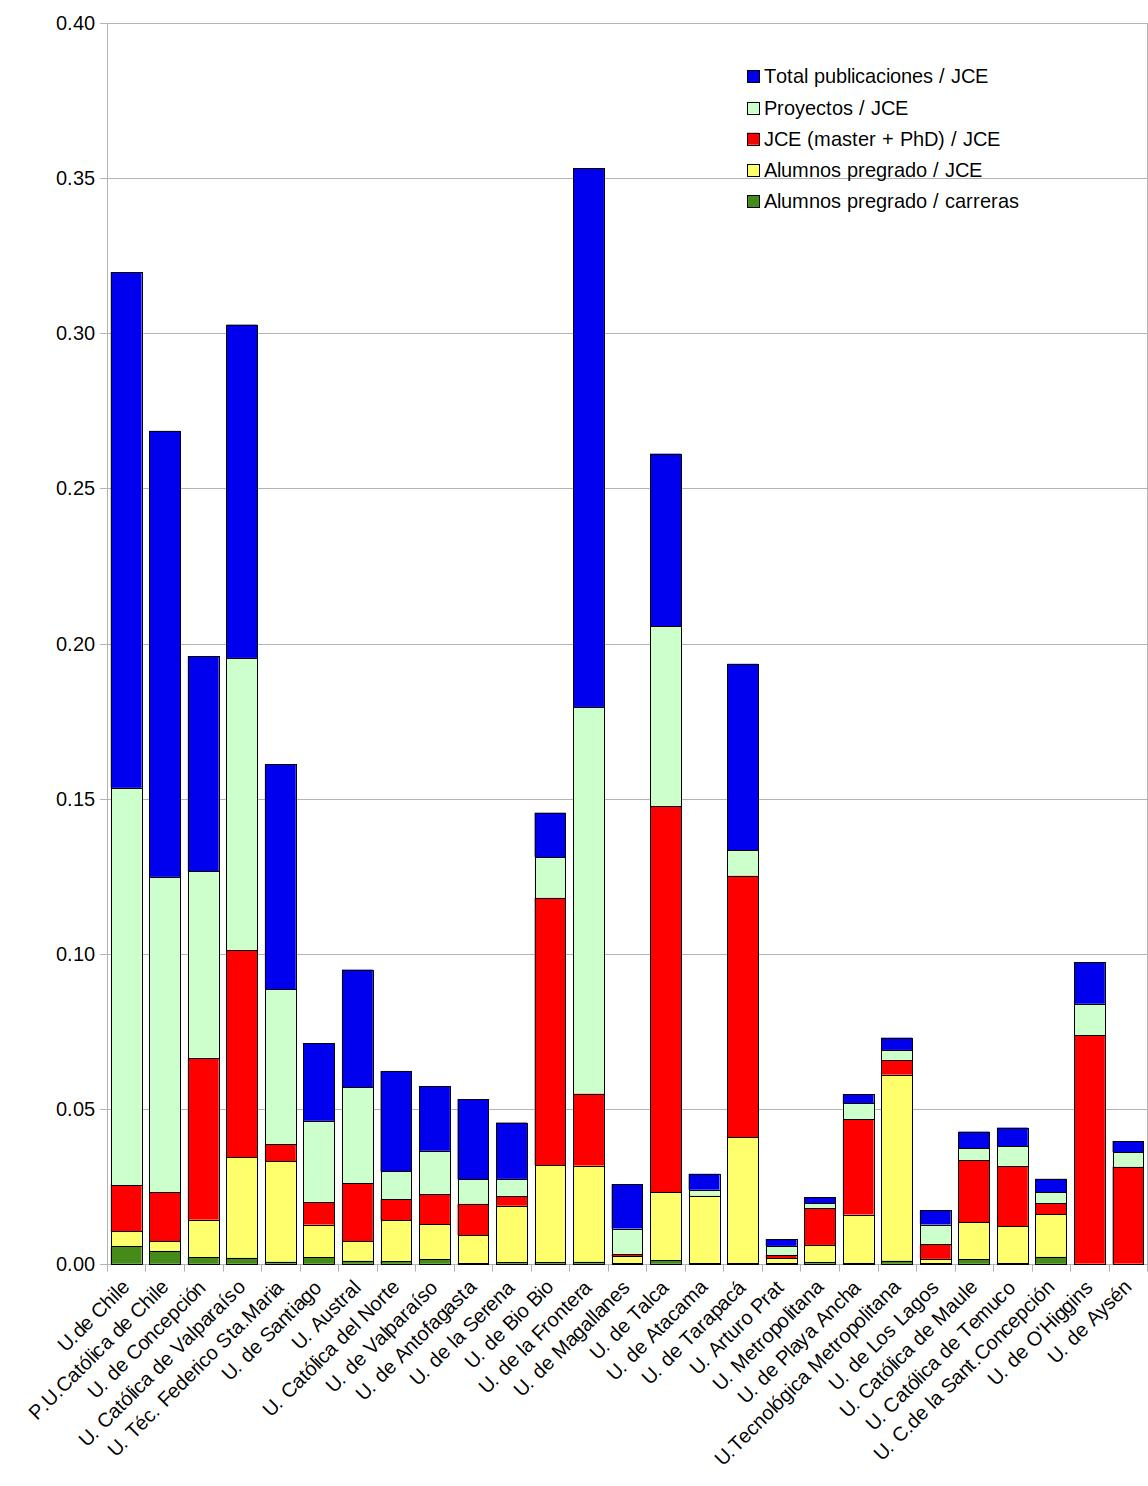
\includegraphics[width=\linewidth]{pdf/afd-coefficients-2018.jpg}
\caption{Graphical representation of the contributions of each AFD coefficient ($c_k y_k$) to each University's score.}
\end{figure*}

\section*{Bibliography}
\bibliographystyle{plainnat}
\bibliography{afd}

\end{document}
